\documentclass[a4paper]{article}
\usepackage{geometry}
\usepackage{graphicx}
\usepackage{natbib}
\usepackage{amsmath}
\usepackage{amssymb}
\usepackage{amsthm}
\usepackage{paralist}
\usepackage{epstopdf}
\usepackage{tabularx}
\usepackage{longtable}
\usepackage{multirow}
\usepackage{multicol}
\usepackage[hidelinks]{hyperref}
\usepackage{fancyvrb}
\usepackage{algorithm}
\usepackage{algorithmic}
\usepackage{float}
\usepackage{paralist}
\usepackage[svgname]{xcolor}
\usepackage{enumerate}
\usepackage{array}
\usepackage{times}
\usepackage{url}
\usepackage{fancyhdr}
\usepackage{comment}
\usepackage{environ}
\usepackage{times}
\usepackage{textcomp}
\usepackage{caption}
\usepackage{color}
\usepackage{xcolor}
\usepackage{qtree}
\usepackage{tikz}
\usepackage{rotating}
\usepackage{subcaption}
\usepackage{listings}
\captionsetup{compatibility=false}

\urlstyle{rm}

\setlength\parindent{0pt} % Removes all indentation from paragraphs
\theoremstyle{definition}
\newtheorem{definition}{Definition}[]
\newtheorem{conjecture}{Conjecture}[]
\newtheorem{example}{Example}[]
\newtheorem{theorem}{Theorem}[]
\newtheorem{lemma}{Lemma}
\newtheorem{proposition}{Proposition}
\newtheorem{corollary}{Corollary}

\floatname{algorithm}{Procedure}
\renewcommand{\algorithmicrequire}{\textbf{Input:}}
\renewcommand{\algorithmicensure}{\textbf{Output:}}
\newcommand{\abs}[1]{\lvert#1\rvert}
\newcommand{\norm}[1]{\lVert#1\rVert}
\newcommand{\RR}{\mathbb{R}}
\newcommand{\CC}{\mathbb{C}}
\newcommand{\Nat}{\mathbb{N}}
\newcommand{\br}[1]{\{#1\}}
\DeclareMathOperator*{\argmin}{arg\,min}
\DeclareMathOperator*{\argmax}{arg\,max}
\renewcommand{\qedsymbol}{$\blacksquare$}

\definecolor{dkgreen}{rgb}{0,0.6,0}
\definecolor{gray}{rgb}{0.5,0.5,0.5}
\definecolor{mauve}{rgb}{0.58,0,0.82}

\newcommand{\Var}{\mathrm{Var}}
\newcommand{\Cov}{\mathrm{Cov}}

\newcommand{\vc}[1]{\boldsymbol{#1}}
\newcommand{\xv}{\vc{x}}
\newcommand{\Sigmav}{\vc{\Sigma}}
\newcommand{\alphav}{\vc{\alpha}}
\newcommand{\muv}{\vc{\mu}}

\newcommand{\red}[1]{\textcolor{red}{#1}}

\def\x{\mathbf x}
\def\y{\mathbf y}
\def\w{\mathbf w}
\def\v{\mathbf v}
\def\E{\mathbb E}
\def\V{\mathbb V}

% TO SHOW SOLUTIONS, include following (else comment out):
\newenvironment{soln}{
    \leavevmode\color{blue}\ignorespaces
}{}


\hypersetup{
%    colorlinks,
    linkcolor={red!50!black},
    citecolor={blue!50!black},
    urlcolor={blue!80!black}
}

\geometry{
  top=1in,            % <-- you want to adjust this
  inner=1in,
  outer=1in,
  bottom=1in,
  headheight=3em,       % <-- and this
  headsep=2em,          % <-- and this
  footskip=3em,
}


\pagestyle{fancyplain}
\lhead{\fancyplain{}{Homework 2}}
\rhead{\fancyplain{}{CS 760 Machine Learning}}
\cfoot{\thepage}

\title{\textsc{Homework 2}} % Title

%%% NOTE:  Replace 'NAME HERE' etc., and delete any "\red{}" wrappers (so it won't show up as red)

\author{
Saikumar Yadugiri \\
saikumar@cs.wisc.edu, 9083079468\\
} 

\date{}

\begin{document}

\maketitle 


\textbf{Instructions:} 
Use this latex file as a template to develop your homework. Submit your homework on time as a single pdf file to Canvas. Please wrap your code and upload to a public GitHub repo, then attach the link below the instructions so that we can access it. You can choose any programming language (i.e. python, R, or MATLAB), as long as you implement the algorithm from scratch (e.g. do not use sklearn on questions 1 to 7 in section 2). Please check Piazza for updates about the homework.

\paragraph{GitHub Link:} \href{https://github.com/saikumarysk/cs760_hw2}{\texttt{https://github.com/saikumarysk/cs760\_hw2}}

\section{A Simplified Decision Tree}
You are to implement a decision-tree learner for classification.
To simplify your work, this will not be a general purpose decision tree.  Instead, your program can assume that
\begin{itemize}
\item each item has two continuous features $\x \in \RR^2$
\item the class label is binary and encoded as $y \in \{0,1\}$
\item data files are in plaintext with one labeled item per line, separated by whitespace:
$$x_{11} \quad x_{12} \quad y_1$$
$$...$$
$$x_{n1} \quad x_{n2} \quad y_n$$
\end{itemize}

Your program should implement a decision tree learner according to the following guidelines:
\begin{itemize}
\item Candidate splits $(j,c)$ for numeric features should use a threshold $c$ in feature dimension $j$ in the form of $x_{j}\ge c$.
\item $c$ should be on values of that dimension present in the training data; i.e. the threshold is on training points, not in between training points. You may enumerate all features, and for each feature, use all possible values for that dimension.
\item You may skip those candidate splits with zero split information (i.e. the entropy of the split), and continue the enumeration.
\item The left branch of such a split is the ``then'' branch, and the right branch is ``else''.
\item Splits should be chosen using information gain ratio. If there is a tie you may break it arbitrarily.
\item The stopping criteria (for making a node into a leaf) are that 
	\begin{itemize}
	\item the node is empty, or
	\item all splits have zero gain ratio (if the entropy of the split is non-zero), or
	\item the entropy of any candidates split is zero
	\end{itemize}
\item To simplify, whenever there is no majority class in a leaf, let it predict $y=1$.
\end{itemize}

\section{Questions}
\begin{enumerate}
\item (Our algorithm stops at pure labels) [10 pts] If a node is not empty but contains training items with the same label, why is it guaranteed to become a leaf?  Explain. You may assume that the feature values of these items are not all the same. \\

\begin{soln}
    As all the labels are the same, the entropy of $Y$ is zero, i.e, $H_{D}(Y) = 0$.
    Moreover, no matter how we split, the value of $Y$ will be same. That is, given the splitting information $S$, the uncertainity in $Y$ still remains 0.
    So, $H_D(Y | S) = 0$.
    Hence, the information gain ratio is 0 for any split which is a stopping criterion in the design of our Decision Tree algorithm.
    So, a non-empty node with all training items having same label will become a leaf.
\end{soln}

\item (Our algorithm is greedy)  [10 pts] Handcraft a small training set where both classes are present but the algorithm refuses to split; instead it makes the root a leaf and stop;
Importantly, if we were to manually force a split, the algorithm will happily continue splitting the data set further and produce a deeper tree with zero training error.
You should (1) plot your training set, (2) explain why.  Hint: you don't need more than a handful of items. \\

\begin{soln}
    Consider the complete XOR ($\oplus$) data set, i.e, $Y = X_1 \oplus X_2$ for every possible $X_1$ and $X_2$ ($\mathsf{Dxor.txt}$).
    Here, we can see that $H_D(Y) = 1$.
    And, for any possible split, the information gain will be zero.
    In other words, for any possible split $S$, $H_D(Y | S) = 1$.
    For instance, consider the split $X_1 \geq 1$.
    We have that $H_D(Y | X_1 \geq 1) = 1$ and $H_D(Y | X_1 < 1) = 1$.
    Hence, $H_D(Y | S) = \frac{1}{2} \times 1 + \frac{1}{2} \times 1 = 1$.
    Similarly all other possible splits give zero information gain.
    So, the decision tree algorithm refuses to split and sets the root node to $T$ and halts.
    However if we manually force a split, every data point will be a leaf node on its own.

    \begin{figure}[h]
        \centering
        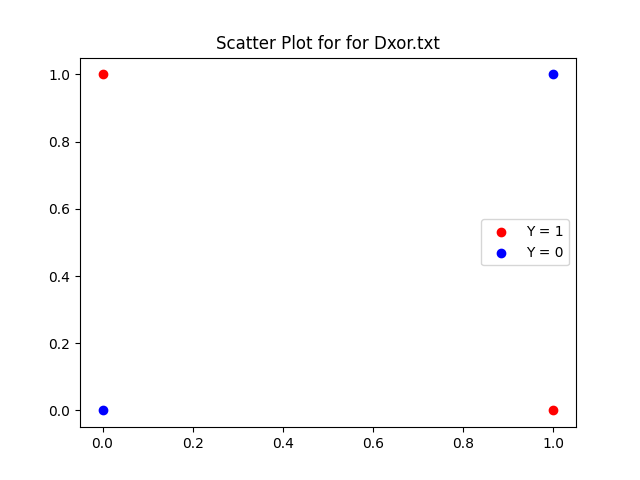
\includegraphics[width=0.75\linewidth]{Scatter_Dxor.png}
        \caption{Scatter Plot for $\mathsf{Dxor.txt}$}
        \label{fig:1}
    \end{figure}
\end{soln}

\item (Information gain ratio exercise)  [10 pts] Use the training set Druns.txt.  For the root node, list all candidate cuts and their information gain ratio. If the entropy of the candidate split is zero, please list its mutual information (i.e. information gain). Hint: to get $\log_2(x)$ when your programming language may be using a different base, use \verb|log(x)/log(2)|. Also, please follow the split rule in the first section. \\

\begin{soln}
    The required information can be found in table \ref{tab:1}. My code doesn't explicitly provide these values. I had to use some debugging statements and workarounds to get these values.

    \begin{table}[H]
        \centering
        \begin{tabular}{|c|c|c|c|}
           \hline
           \textbf{Feature} & \textbf{Threshold (c)} & $\mathbf{H_{D}(S)}$ & \textbf{Information Gain Ratio}\\
           \hline
           $X_1$ & 0 & 0 & 0 \\
           \hline
           $X_1$ & 0.1 & 0.4395 & 0.10052 \\
           \hline
           $X_2$ & -1 & 0.4395 & 0.10052 \\
           \hline
           $X_2$ & 0 & 0.68404 & 0.05596 \\
           \hline
           $X_2$ & 6 & 0.84535 & 0.2361 \\
           \hline
           $X_2$ & 7 & 0.68404 & 0.05596 \\
           \hline
           $X_2$ & 8 & 0.4395 & 0.43015 \\
           \hline
        \end{tabular}
        \caption{Split Information for the root node in $\mathsf{Druns.txt}$}
        \label{tab:1}
    \end{table}
    
\end{soln}

\item (The king of interpretability)  [10 pts] Decision tree is not the most accurate classifier in general.  However, it persists.  This is largely due to its rumored interpretability: a data scientist can easily explain a tree to a non-data scientist.  Build a tree from D3leaves.txt.  Then manually convert your tree to a set of logic rules.  Show the tree\footnote{When we say show the tree, we mean either the standard computer science tree view, or some crude plaintext representation of the tree -- as long as you explain the format.  When we say visualize the tree, we mean a plot in the 2D $\x$ space that shows how the tree will classify any points.} and the rules. \\

\begin{soln}
    The tree resulted from my code is shown in figure \ref{fig:2}.
    \begin{figure}[H]
        \centering
        \begin{tikzpicture}
            \node (root) at (0, 0) {$X_2 \geq 2$};
            \node (left1) at (-1, -1) {1};
            \node (right1) at (1, -1) {$X_1 \geq 10$};
            \node (left2) at (0, -2) {1};
            \node (right2) at (2, -2) {0};

            \node (T1) at (-0.75, -0.35) {T};
            \node (F1) at (0.75, -0.35) {F};
            \node (T2) at (0.25, -1.35) {T};
            \node (F2) at (1.75, -1.35) {F};

            \draw[-latex] (root) -- (left1);
            \draw[-latex] (root) -- (right1);
            \draw[-latex] (right1) -- (left2);
            \draw[-latex] (right1) -- (right2);
        \end{tikzpicture}
        \caption{Decision Tree for $\mathsf{D3leaves.txt}$}
        \label{fig:2}
    \end{figure}

    It's logical formula is $(X_2 \geq 2) \vee (X_1 \geq 10)$ where $X_i$ is the $i$-th feature.
    
\end{soln}

\item (Or is it?)  [10 pts] For this question only, make sure you DO NOT VISUALIZE the data sets or plot your tree's decision boundary in the 2D $\x$ space.  If your code does that, turn it off before proceeding.  This is because you want to see your own reaction when trying to interpret a tree.  You will get points no matter what your interpretation is.
And we will ask you to visualize them in the next question anyway.
  \begin{itemize}
  
  \item Build a decision tree on D1.txt.  Show it to us in any format (e.g. could be a standard binary tree with nodes and arrows, and denote the rule at each leaf node; or as simple as plaintext output where each line represents a node with appropriate line number pointers to child nodes; whatever is convenient for you). Again, do not visualize the data set or the tree in the $\x$ input space.  In real tasks you will not be able to visualize the whole high dimensional input space anyway, so we don't want you to ``cheat'' here. 

  \begin{soln}
      The decision tree resulted from my code is shown in figure \ref{fig:3}.

      \begin{figure}[H]
          \centering
          \begin{tikzpicture}
            \node (root) at (0, 0) {$X_2 \geq 0.201829$};
            \node (left1) at (-1, -1) {1};
            \node (right1) at (1, -1) {0};

            \node (T1) at (-0.75, -0.35) {T};
            \node (F1) at (0.75, -0.35) {F};

            \draw[-latex] (root) -- (left1);
            \draw[-latex] (root) -- (right1);
          \end{tikzpicture}
          \caption{Decision Tree for $\mathsf{D1.txt}$}
          \label{fig:3}
      \end{figure}
  \end{soln}
  
  \item Look at your tree in the above format (remember, you should not visualize the 2D dataset or your tree's decision boundary) and try to interpret the decision boundary in human understandable English.
  \begin{soln}
      The decision boundary will be a horizontal straight line in the $(X_1, X_2)$ plane where the $X_2$-intercept will be 0.201829 and the $X_1$ intercept is $\infty$.
  \end{soln}
  
  \item Build a decision tree on D2.txt.  Show it to us.\\
  \begin{soln}
      The decision tree resulted from my code is shown in the following tree (it's the horizontal page).
       \begin{sidewaysfigure}
       { \tiny
      \Tree[.{$X_1 \geq 0.533076$} 
            [.{$X_2 \geq 0.228007$}
                [.{$X_2 \geq 0.424906$}
                    [.1 ]
                    [.{$X_1 \geq 0.701827$}
                       [.1 ]
                       [.{$X_2 \geq 0.32625$}
                            [.{$X_1 \geq 0.595471$}
                                [.{$X_1 \geq 0.646007$}
                                    [.1 ]
                                    [.{$X_2 \geq 0.403494$}
                                        [.1 ]
                                        [.0 ]
                                    ]
                                ]
                                [.0 ]
                            ]
                            [.0 ]
                       ]
                    ]
                ] 
                [.{$X_1 \geq 0.887224$}
                    [.{$X_2 \geq 0.037708$}
                        [.{$X_2 \geq 0.082895$}
                            [.1 ]
                            [.{$X_1 \geq 0.960783$}
                                [.1 ]
                                [.0 ]
                            ]
                        ]
                        [.0 ]
                    ]
                    [.{$X_1 \geq 0.850316$}
                        [.{$X_2 \geq 0.169053$}
                            [.1 ]
                            [.0 ]
                        ]
                        [.0 ]
                    ]
                ] 
            ]
            [.{$X_2 \geq 0.88635$}
                [.{$X_1 \geq 0.041245$}
                    [.{$X_1 \geq 0.104043$}
                        [.1 ]
                        [.{$X_2 \geq 0.964767$}
                            [.1 ]
                            [.0 ]
                        ]
                    ]
                    [.0 ]
                ]
                [.{$X_2 \geq 0.691474$}
                    [.{$X_1 \geq 0.254049$}
                        [.1 ]
                        [.{$X_1 \geq 0.191915$}
                            [.{$X_2 \geq 0.792752$}
                               [.1 ]
                               [.0 ]
                            ]
                            [.{$X_2 \geq 0.864128$}
                                [.{$X_2 \geq 0.865999$}
                                    [.0 ]
                                    [.1 ]
                                ]
                                [.0 ]
                            ]
                        ]
                    ]
                    [.{$X_2 \geq 0.534979$}
                        [.{$X_1 \geq 0.426073$}
                            [.1 ]
                            [.{$X_1 \geq 0.409972$}
                                [.{$X_2 \geq 0.597713$}
                                    [.1 ]
                                    [.0 ]
                                ]
                                [.{$X_1 \geq 0.393227$}
                                    [.{$X_2 \geq 0.639018$}
                                        [.1 ]
                                        [.0 ]
                                    ]
                                    [.0 ]
                                ]
                            ]
                        ]
                        [.0 ]
                    ]
                ]
            ]
    ]
    }
    \end{sidewaysfigure}
    \end{soln}
  
  \item Try to interpret your D2 decision tree. Is it easy or possible to do so without visualization? \\
  \begin{soln}
      We can interpret the decision tree as an SMT constraint but it is quite long.
      It is certainly hard without visualizing the tree.
      Something like this:
      \begin{center}
          $( X_1 \geq 0.533076 \wedge X_2 \geq 0.424906 ) \vee ( 0.228007 \leq X_2 < 0.424906 \wedge X_1 \geq 0.701827 ) \  \vee$ \\
          $( 0.646007 \leq X_1 < 0.701827 \wedge 0.32625 \leq X_2 < 0.424906 ) \vee$ \\
          $( 0.595471 \leq X_1 < 0.646007 \wedge 0.403494 \leq X_2 < 0.424906 ) \vee$ \\
          $( X_1 \geq 0.887224 \wedge 0.082895 \leq X_2 < 0.228007 ) \vee ( X_1 \geq 0.960783 \wedge 0.037708 \leq X_2 < 0.082895 ) \vee$ \\
          $( 0.850316 \leq X_1 < 0.887224 \wedge X_2 \geq 0.228007 ) \vee ( 0.104043 \leq X_1 < 0.533076 \wedge X_2 \geq 0.88635 ) \vee$ \\
          $( 0.041245 \leq X_1 < 0.104043 \wedge X_2 \geq 0.964767 ) \vee$ \\
          $( 0.254049 \leq X_1 < 0.533076 \wedge 0.691474 \leq X_2 < 0.88635 ) \vee$
          $( 0.191915 \leq X_1 < 0.254049 \wedge 0.792752 \leq X_2 < 0.88635 ) \vee$\\
          $( X_1 < 0.191915 \wedge 0.864128 \leq X_2 < 0.865999 ) \vee ( X_1 < 0.191915 \wedge 0.864128 \leq X_2 < 0.865999 ) \vee$ \\
          $( 0.426073 \leq X_1 < 0.533076 \wedge 0.534979 \leq X_2 < 0.691474 ) \vee$\\
          $( 0.191915 \leq X_1 < 0.254049 \wedge 0.792752 \leq X_2 < 0.88635 ) \vee$\\
          $( 0.409977 \leq X_1 < 0.426073 \wedge 0.597713 \leq X_2 < 0.691474 ) \vee$\\
          $( 0.393227 \leq X_1 < 0.409972 \wedge 0.639018 \leq X_2 < 0.691474 ) \vee$\\
      \end{center}
  \end{soln}
  \end{itemize}

\item (Hypothesis space)  [10 pts] For D1.txt and D2.txt, do the following separately:
  \begin{itemize}
  
  \item Produce a scatter plot of the data set.

  \begin{soln}
      The scatter plots are shown in figure \ref{fig:4}.

      \begin{figure}[H]
          \centering
          \begin{subfigure}{0.5\textwidth}
          \centering
          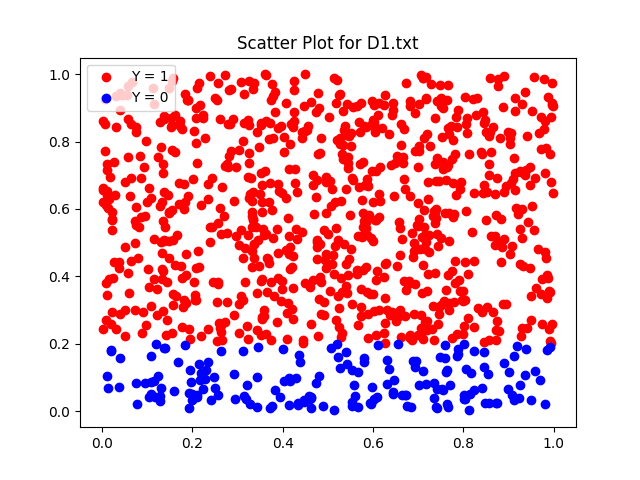
\includegraphics[width=1.1\linewidth]{Scatter_D_1.png}
          \caption{$\mathsf{D1.txt}$}
          \label{fig:3sub1}
        \end{subfigure}%
        \begin{subfigure}{0.5\textwidth}
          \centering
          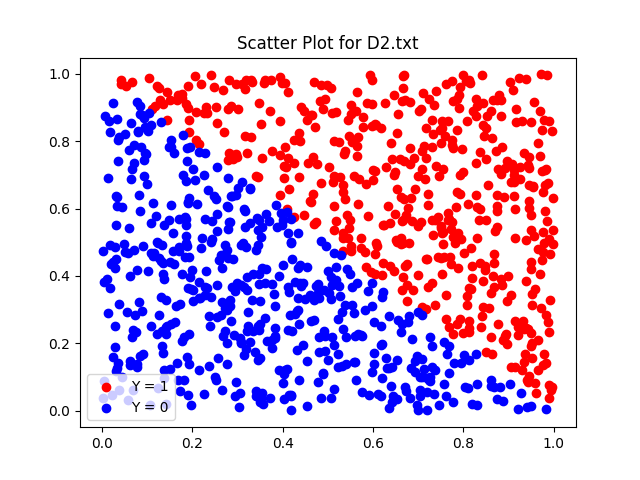
\includegraphics[width=1.1\linewidth]{Scatter_D_2.png}
          \caption{$\mathsf{D2.txt}$}
          \label{fig:3sub2}
          \end{subfigure}
          \caption{Scatter Plots for $\mathsf{D1.txt}$ and $\mathsf{D2.txt}$}
          \label{fig:4}
      \end{figure}
  \end{soln}

  \item Visualize your decision tree's decision boundary (or decision region, or some other ways to clearly visualize how your decision tree will make decisions in the feature space).

  \begin{soln}
      The decision boundaries are shown in figure \ref{fig:5}.

      \begin{figure}[H]
          \centering
          \begin{subfigure}{0.5\textwidth}
          \centering
          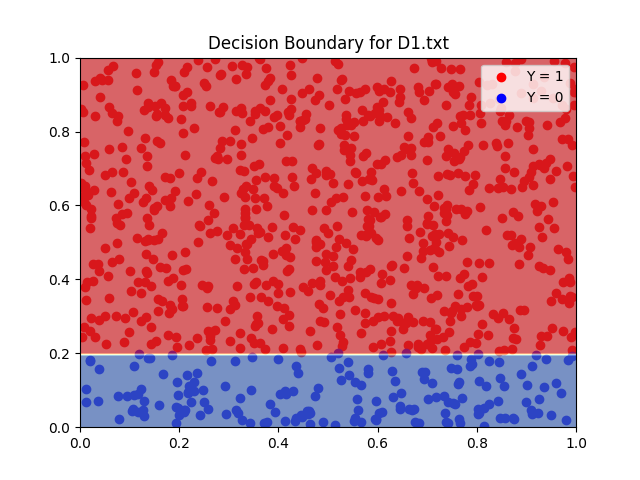
\includegraphics[width=1.1\linewidth]{Decision_Boundary_D1.png}
          \caption{$\mathsf{D1.txt}$}
          \label{fig:5sub1}
        \end{subfigure}%
        \begin{subfigure}{0.5\textwidth}
          \centering
          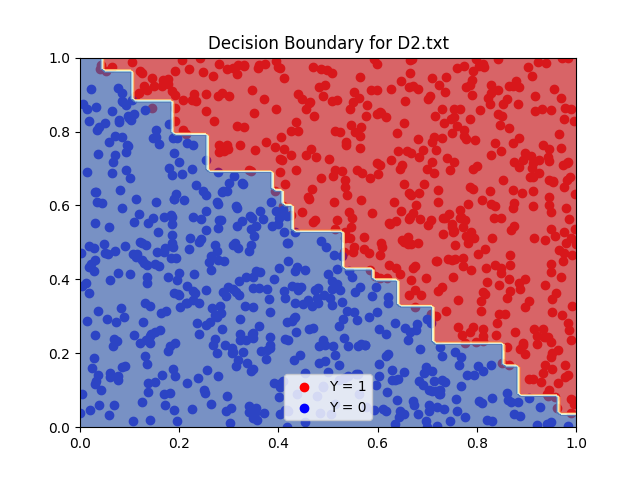
\includegraphics[width=1.1\linewidth]{Decision_Boundary_D2.png}
          \caption{$\mathsf{D2.txt}$}
          \label{fig:5sub2}
          \end{subfigure}
          \caption{Approximate Decision Boundaries for $\mathsf{D1.txt}$ and $\mathsf{D2.txt}$}
          \label{fig:5}
      \end{figure}
  \end{soln}

  \end{itemize}
Then discuss why the size of your decision trees on D1 and D2 differ.  Relate this to the hypothesis space of our decision tree algorithm. \\

\begin{soln}
    For the data in $\mathsf{D1.txt}$, the decision entirely depends on one of the feature, $X_2$. However, for $\mathsf{D2.txt}$, we need to infer information from both $X_1$ and $X_2$ in a single node to predict accurately. That is, if we have a node whose split condition is like $X_1 + X_2 \geq 1$, then we can get a tree which looks like the decision tree for $\mathsf{D1.txt}$.

    But, we are generating the decision tree by considering one feature per node, as dictated by the hypothesis bias of the decision tree learning method. Hence, $\mathsf{D1.txt}$ gives a shorter, accurate tree whereas $\mathsf{D2.txt}$ gives a complicated tree. The decision boundary for $\mathsf{D2.txt}$'s decision tree hypothesis will contain a lot of horizontal and vertical lines near the line $X_1 + X_2 = 1$. If we get more training instances near the said line, we can be more accurately picture the decision boundary at the cost of a deeper decision tree and higher testing time.
\end{soln}

\item (Learning curve)  [20 pts] We provide a data set Dbig.txt with 10000 labeled items.  Caution: Dbig.txt is sorted.
  \begin{itemize}
  
  \item You will randomly split Dbig.txt into a candidate training set of 8192 items and a test set (the rest).  Do this by generating a random permutation, and split at 8192.
  
  \item Generate a sequence of five nested training sets $D_{32} \subset D_{128} \subset D_{512} \subset D_{2048} \subset D_{8192}$ from the candidate training set.  The subscript $n$ in $D_n$ denotes training set size.  The easiest way is to take the first $n$ items from the (same) permutation above.  This sequence simulates the real world situation where you obtain more and more training data.
  
  \item For each $D_n$ above, train a decision tree.  Measure its test set error $err_n$.  Show three things in your answer: (1) List $n$, number of nodes in that tree, $err_n$. (2) Plot $n$ vs. $err_n$.  This is known as a learning curve (a single plot). (3) Visualize your decision trees' decision boundary (five plots). \\
  \end{itemize}

  \begin{soln}
      The nodes generated by my code and the $err_n$ information is provided in the tabular form in table \ref{tab:2} and the plot is shown in \ref{fig:6}.
      The decision boundaries are shown in figure \ref{fig:7}.

      \begin{table}[H]
          \centering
          \begin{tabular}{|c|c|c|}
              \hline
              $\mathbf{n}$ & \textbf{\# of nodes} & $\mathbf{err_n}$ \\
              \hline
              32 & 9 & 0.14767 \\
              \hline
              128 & 17 & 0.10896 \\
              \hline
              512 & 49 & 0.05862 \\
              \hline
              2048 & 139 & 0.03207 \\
              \hline
              8192 & 309 & 0.01493 \\
              \hline
          \end{tabular}
          \caption{Number of nodes for each $n$}
          \label{tab:2}
      \end{table}

    \begin{figure}[H]
        \centering
        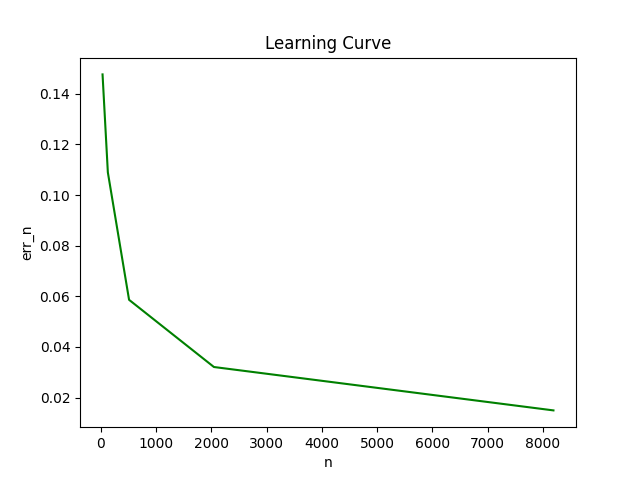
\includegraphics[width=0.65\textwidth]{err_n.png}
        \caption{Learning Curve for Decision Tree by my code}
        \label{fig:6}
    \end{figure}

    \begin{figure}[H]
          \centering
          \begin{subfigure}{0.5\textwidth}
          \centering
          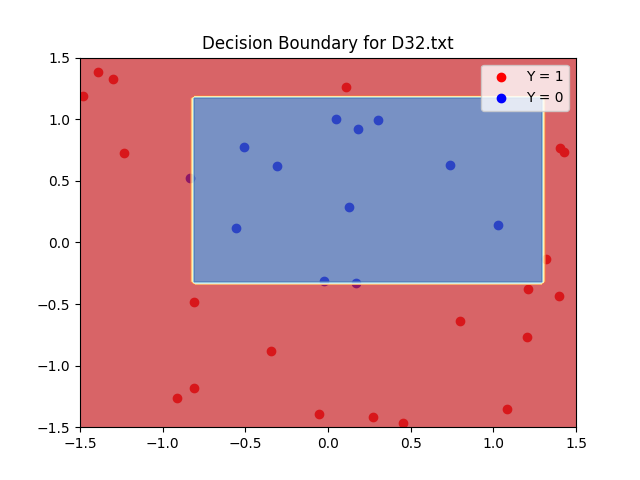
\includegraphics[width=1.1\linewidth]{Decision_Boundary_D32.png}
          \caption{$\mathsf{D32.txt}$}
          \label{fig:7sub1}
        \end{subfigure}%
        \begin{subfigure}{0.5\textwidth}
          \centering
          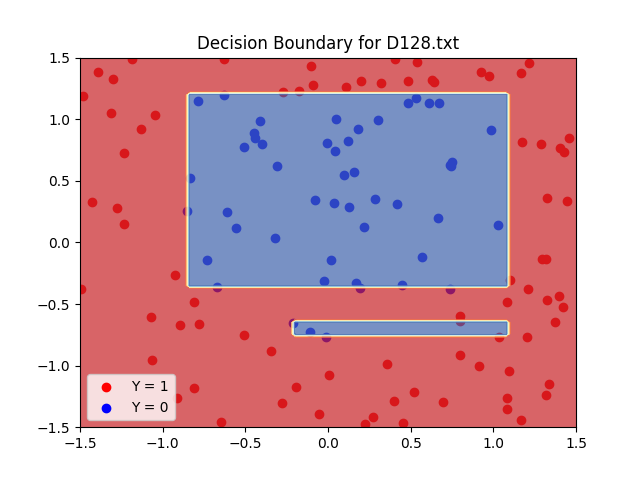
\includegraphics[width=1.1\linewidth]{Decision_Boundary_D128.png}
          \caption{$\mathsf{D128.txt}$}
          \label{fig:7sub2}
          \end{subfigure}
          \begin{subfigure}{0.5\textwidth}
          \centering
          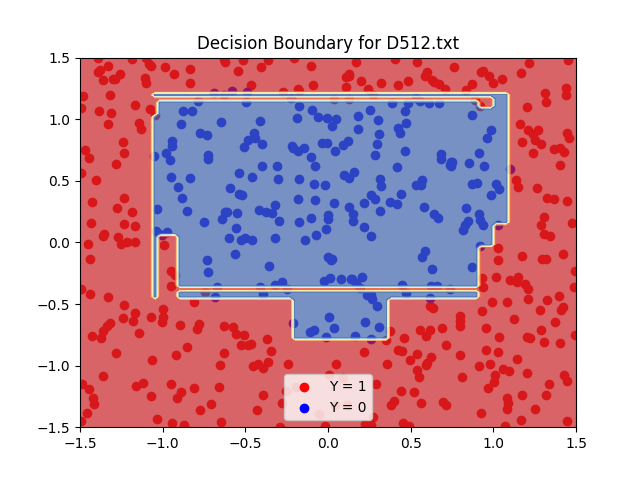
\includegraphics[width=1.1\linewidth]{Decision_Boundary_D512.png}
          \caption{$\mathsf{D512.txt}$}
          \label{fig:7sub3}
        \end{subfigure}%
        \begin{subfigure}{0.5\textwidth}
          \centering
          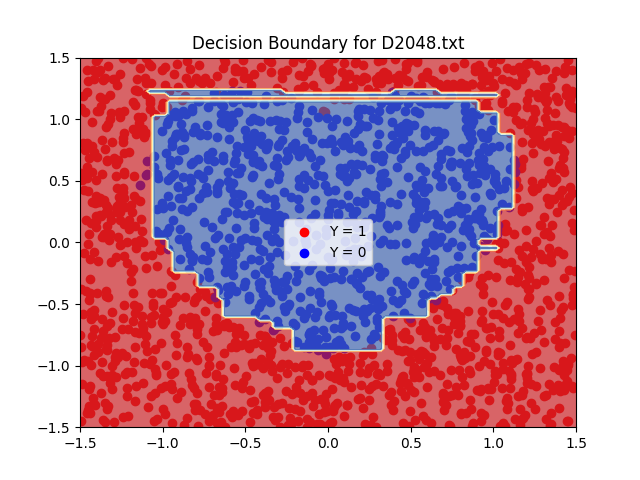
\includegraphics[width=1.1\linewidth]{Decision_Boundary_D2048.png}
          \caption{$\mathsf{D2048.txt}$}
          \label{fig:7sub4}
          \end{subfigure}
          \centering
          \begin{subfigure}{0.5\textwidth}
          \centering
          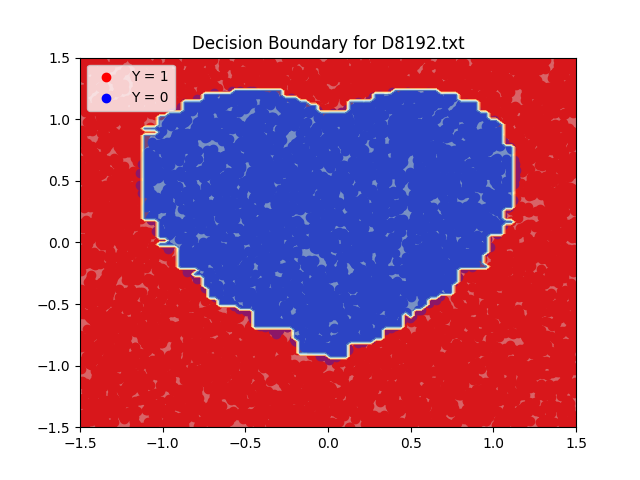
\includegraphics[width=1.1\linewidth]{Decision_Boundary_D8192.png}
          \caption{$\mathsf{D8192.txt}$}
          \label{fig:7sub5}
          \end{subfigure}%
          \caption{Approximate Decision Boundaries for $\mathsf{D32.txt}$, $\mathsf{D128.txt}$, $\mathsf{D512.txt}$, $\mathsf{D2048.txt}$, and $\mathsf{D8192.txt}$}
          \label{fig:7}
      \end{figure}
  \end{soln}
  
\end{enumerate}

\section{sklearn [10 pts]}
Learn to use sklearn (\url{https://scikit-learn.org/stable/}).
Use sklearn.tree.DecisionTreeClassifier to produce trees for datasets $D_{32}, D_{128}, D_{512}, D_{2048}, D_{8192}$.  Show two things in your answer: (1) List $n$, number of nodes in that tree, $err_n$. (2) Plot $n$ vs. $err_n$.

\begin{soln}
      The nodes generated by my code and the $err_n$ information is provided in the tabular form in table \ref{tab:3} and the plot is shown in figure \ref{fig:8}.

      \begin{table}[H]
          \centering
          \begin{tabular}{|c|c|c|}
              \hline
              $\mathbf{n}$ & \textbf{\# of nodes} & $\mathbf{err_n}$ \\
              \hline
              32 & 9 & 0.10674 \\
              \hline
              128 & 15 & 0.11559 \\
              \hline
              512 & 41 & 0.04480 \\
              \hline
              2048 & 125 & 0.03097 \\
              \hline
              8192 & 237 & 0.00940 \\
              \hline
          \end{tabular}
          \caption{Number of nodes for each $n$ for \textsf{sklearn}}
          \label{tab:3}
      \end{table}

    \begin{figure}[H]
        \centering
        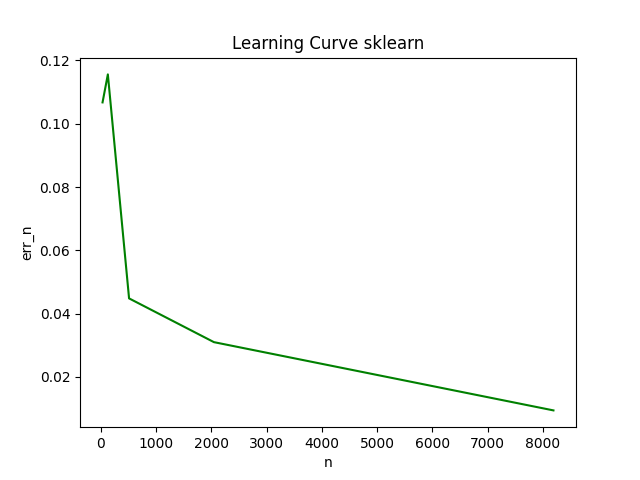
\includegraphics[width=0.65\textwidth]{err_n_sklearn.png}
        \caption{Learning Curve for Decision Tree by \textsf{sklearn}}
        \label{fig:8}
    \end{figure}

    \paragraph{Note:} \textsf{sklearn} uses random selection. So, I ran each $n$ multiple times and took the smallest error possible. I used \textsf{sklearn} version 1.3.0.
  \end{soln}

\section{Lagrange Interpolation [10 pts]}
Fix some interval $[a, b]$ and sample $n = 100$ points $x$ from this interval uniformly. Use these to build a training set consisting of $n$ pairs $(x, y)$ by setting function $y = sin(x)$. \\

Build a model $f$ by using Lagrange interpolation, check more details in \url{https://en.wikipedia.org/wiki/Lagrange_polynomial} and \url{https://docs.scipy.org/doc/scipy/reference/generated/scipy.interpolate.lagrange.html}. \\

Generate a test set using the same distribution as your training set. Compute and report the model’s train and test \textbf{log mean squared error}. What do you observe? Repeat the experiment with zero-mean Gaussian noise added to x \textbf{when creating the training set}, i.e, points are now $(x + \epsilon, \sin(x + epsilon))$. \textbf{The test set remains the same}. Vary the standard deviation for epsilon and report your findings.

\begin{soln}
    For this question, I chose $n = 400$ samples from $[a, b] = [0, 4]$ as my test data.
    The data is present in $\mathsf{Dsin.txt}$ in the same format as data files from section 2.
    I built the Lagrange polynomial and my training error was 0.0.
    This is because the training will fit a polynomial that goes through all of the $(x, y)$ in the training data \footnote{The model doesn't require a training phase as you can directly test using the training values, similar to k-NN learning model.}.
    Thus all the points are accurately predicted by the Lagrange polynomial.
    Hence, training error is expected to be 0.
    The testing error I got was $\log_{10}(2.3991067263715886e+40) = 40.38005$ which is very high.
    This is because the polynomial might not go through all the points on the sine curve as the Taylor-series expansion of sine curve is an infinite polynomial.

    In the next part of the experiment, I sampled $x$ from an uniform distribution from $[0, 4]$ and the error from a zero-mean Gaussian distribution.
    I varied the standard deviation from $\sigma = 0.1 \text{ to } \sigma = 3$ in irregular steps and set $y = \sin(x)$, where $x$ implicitly includes the zero-mean Gaussian error.
    The training error remained zero (as expected) in all variations of $\sigma$.
    However, the testing error decreased dramatically as the data deviated from the $\sin$-curve distribution and become less comprehensible.
    I used the same testing set as the previous experiment as mentioned in the 
    The results are produced in the table \ref{tab:4}.
    The plot is provided in figure \ref{fig:9}.

    \begin{table}[H]
        \centering
        \begin{tabular}{|c|c|c|}
            \hline
            $\mathbf{\sigma}$ & \textbf{Testing Error (MSE)} & \textbf{Testing Error (log-MSE)} \\
            \hline
            0.1 & 4.323348808761835e+34 & 34.63582 \\
            \hline
            0.2 & 6.464341563037188e+61 & 61.81052 \\
            \hline
            0.3 & 2.1122050373236405e+40 & 40.32474 \\
            \hline
            0.5 & 1.7255371955631576e+37 & 37.23692 \\
            \hline
            0.7 & 7.247605580034653e+51 & 51.86019 \\
            \hline
            0.9 & 6.160835860455152e+30 & 30.78964 \\
            \hline
            1 & 2.34853471287732e+30 & 30.3708\\
            \hline
            1.5 & 3.947203987693241e+17 & 17.59629 \\
            \hline
            2 & 0.0006167642993747171 & -3.20988 \\
            \hline
            2.5 & 1.1984034812979894e-06 & -5.9214 \\
            \hline
            3 & 1.377963569529834e-05 & -4.86076 \\ 
            \hline
        \end{tabular}
        \caption{Standard Deviation vs. Testing Error for Lagrange Interpolation of Noisy $\sin$ data}
        \label{tab:4}
    \end{table}

    \begin{figure}[H]
        \centering
        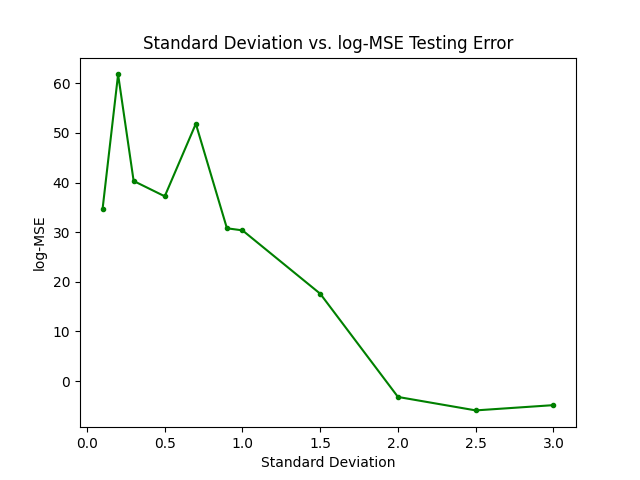
\includegraphics[width=0.75\linewidth]{logMSE.png}
        \caption{Standard Deviation vs. log-MSE for Lagrange Interpolation of Noisy $\sin$ data}
        \label{fig:9}
    \end{figure}
\end{soln}

\bibliographystyle{apalike}
\end{document}